\documentclass[a4paper,conference]{IEEEtran}
% This is stripped down to basically the ieee bare_conf.tex header
\usepackage{amssymb,amsmath}
% use upquote if available, for straight quotes in verbatim environments
\IfFileExists{upquote.sty}{\usepackage{upquote}}{}
% use microtype if available
\IfFileExists{microtype.sty}{%
\usepackage{microtype}
\UseMicrotypeSet[protrusion]{basicmath} % disable protrusion for tt fonts
}{}
\usepackage{hyperref}
\PassOptionsToPackage{usenames,dvipsnames}{color} % color is loaded by hyperref
\hypersetup{unicode=true,
            pdftitle={Predicting Portuguese Secondary-School Achievement; An Integrated Data-Mining Study},
            pdfborder={0 0 0},
            breaklinks=true}
\urlstyle{same}  % don't use monospace font for urls
% -- biblio. set natbib: true in pandoc for silly hacks around pandoc \cite{} vs \citep{}
\usepackage{cite}
\bibliographystyle{IEEEtran}
\let\citep\cite
% if you want the [2, 3] vs IEEE [2], [3]
\renewcommand{\citepunct}{,\penalty\citepunctpenalty\ }
\usepackage{color}
\usepackage{fancyvrb}
\newcommand{\VerbBar}{|}
\newcommand{\VERB}{\Verb[commandchars=\\\{\}]}
\DefineVerbatimEnvironment{Highlighting}{Verbatim}{commandchars=\\\{\}}
% Add ',fontsize=\small' for more characters per line
\usepackage{framed}
\definecolor{shadecolor}{RGB}{248,248,248}
\newenvironment{Shaded}{\begin{snugshade}}{\end{snugshade}}
\newcommand{\AlertTok}[1]{\textcolor[rgb]{0.94,0.16,0.16}{#1}}
\newcommand{\AnnotationTok}[1]{\textcolor[rgb]{0.56,0.35,0.01}{\textbf{\textit{#1}}}}
\newcommand{\AttributeTok}[1]{\textcolor[rgb]{0.13,0.29,0.53}{#1}}
\newcommand{\BaseNTok}[1]{\textcolor[rgb]{0.00,0.00,0.81}{#1}}
\newcommand{\BuiltInTok}[1]{#1}
\newcommand{\CharTok}[1]{\textcolor[rgb]{0.31,0.60,0.02}{#1}}
\newcommand{\CommentTok}[1]{\textcolor[rgb]{0.56,0.35,0.01}{\textit{#1}}}
\newcommand{\CommentVarTok}[1]{\textcolor[rgb]{0.56,0.35,0.01}{\textbf{\textit{#1}}}}
\newcommand{\ConstantTok}[1]{\textcolor[rgb]{0.56,0.35,0.01}{#1}}
\newcommand{\ControlFlowTok}[1]{\textcolor[rgb]{0.13,0.29,0.53}{\textbf{#1}}}
\newcommand{\DataTypeTok}[1]{\textcolor[rgb]{0.13,0.29,0.53}{#1}}
\newcommand{\DecValTok}[1]{\textcolor[rgb]{0.00,0.00,0.81}{#1}}
\newcommand{\DocumentationTok}[1]{\textcolor[rgb]{0.56,0.35,0.01}{\textbf{\textit{#1}}}}
\newcommand{\ErrorTok}[1]{\textcolor[rgb]{0.64,0.00,0.00}{\textbf{#1}}}
\newcommand{\ExtensionTok}[1]{#1}
\newcommand{\FloatTok}[1]{\textcolor[rgb]{0.00,0.00,0.81}{#1}}
\newcommand{\FunctionTok}[1]{\textcolor[rgb]{0.13,0.29,0.53}{\textbf{#1}}}
\newcommand{\ImportTok}[1]{#1}
\newcommand{\InformationTok}[1]{\textcolor[rgb]{0.56,0.35,0.01}{\textbf{\textit{#1}}}}
\newcommand{\KeywordTok}[1]{\textcolor[rgb]{0.13,0.29,0.53}{\textbf{#1}}}
\newcommand{\NormalTok}[1]{#1}
\newcommand{\OperatorTok}[1]{\textcolor[rgb]{0.81,0.36,0.00}{\textbf{#1}}}
\newcommand{\OtherTok}[1]{\textcolor[rgb]{0.56,0.35,0.01}{#1}}
\newcommand{\PreprocessorTok}[1]{\textcolor[rgb]{0.56,0.35,0.01}{\textit{#1}}}
\newcommand{\RegionMarkerTok}[1]{#1}
\newcommand{\SpecialCharTok}[1]{\textcolor[rgb]{0.81,0.36,0.00}{\textbf{#1}}}
\newcommand{\SpecialStringTok}[1]{\textcolor[rgb]{0.31,0.60,0.02}{#1}}
\newcommand{\StringTok}[1]{\textcolor[rgb]{0.31,0.60,0.02}{#1}}
\newcommand{\VariableTok}[1]{\textcolor[rgb]{0.00,0.00,0.00}{#1}}
\newcommand{\VerbatimStringTok}[1]{\textcolor[rgb]{0.31,0.60,0.02}{#1}}
\newcommand{\WarningTok}[1]{\textcolor[rgb]{0.56,0.35,0.01}{\textbf{\textit{#1}}}}
\usepackage{graphicx,grffile}
\makeatletter
\def\maxwidth{\ifdim\Gin@nat@width>\linewidth\linewidth\else\Gin@nat@width\fi}
\def\maxheight{\ifdim\Gin@nat@height>\textheight\textheight\else\Gin@nat@height\fi}
\makeatother
% Scale images if necessary, so that they will not overflow the page
% margins by default, and it is still possible to overwrite the defaults
% using explicit options in \includegraphics[width, height, ...]{}
\setkeys{Gin}{width=\maxwidth,height=\maxheight,keepaspectratio}

\title{Predicting Portuguese Secondary-School Achievement; An Integrated
Data-Mining Study}
% for over three affiliations, or if they all won't fit within the width
% of the page, use this alternative format. Cannot use \and or alignment is wrong
\author{\IEEEauthorblockN{%
  Will Marschall\IEEEauthorrefmark{1}\,\IEEEauthorrefmark{2}%
  , Matthew Martin\IEEEauthorrefmark{1}\,\IEEEauthorrefmark{4}%
  , Porter Jurica\IEEEauthorrefmark{1}\,\IEEEauthorrefmark{5}%
}
\IEEEauthorblockA{\IEEEauthorrefmark{1}
      School of Engineering and Applied Science\\
      University of Virginia, Charlottesville, Virginia 22904}
\IEEEauthorblockA{\IEEEauthorrefmark{2}
      Email:
\href{mailto:fmb8ek@virginia.edu}{\nolinkurl{fmb8ek@virginia.edu}}}
\IEEEauthorblockA{\IEEEauthorrefmark{4}
      Email:
\href{mailto:vhs6gh@virginia.edu}{\nolinkurl{vhs6gh@virginia.edu}}}
\IEEEauthorblockA{\IEEEauthorrefmark{5}
      Email:
\href{mailto:wwk7ja@virginia.edu}{\nolinkurl{wwk7ja@virginia.edu}}}
}





\date{2025-07-05 16:42:10 -0400}
\setlength{\parindent}{0pt}
\setlength{\parskip}{6pt plus 2pt minus 1pt}
\let\tightlist\relax % silly pandoc thing

% --- user includes
% ---------------------------------------------------------------
%  PREAMBLE FOR IEEE-STYLE R MARKDOWN PDF (Pandoc ??? 2.19)
% ---------------------------------------------------------------

% ----------  Pandoc & pandoc-crossref support  ----------
\usepackage{adjustbox}              % needed for \pandocbounded
\usepackage{hyperref}
\usepackage[capitalize,nameinlink]{cleveref}

\makeatletter
\def\maxwidth{\ifdim\Gin@nat@width>\linewidth\linewidth\else\Gin@nat@width\fi}
\def\maxheight{\ifdim\Gin@nat@height>\textheight\textheight\else\Gin@nat@height\fi}
\def\pandocbounded#1{%
  \begin{adjustbox}{width=\maxwidth,height=\maxheight,keepaspectratio}#1\end{adjustbox}}
\makeatother
% ----------------------------------------------------------

% ----------  Your original packages and macros  ----------
% subfigures (IEEEtran recommends subcaption over subfig)
\usepackage{subcaption}

% graphics, incl. filenames with dots
\usepackage{graphicx, grffile}

% bold math
\usepackage{bm}

% colours
\usepackage[usenames,dvipsnames]{xcolor}

% math shortcuts
\newcommand{\E}[1]{\operatorname{\mathbb{E}}\!\left[#1\right]}
\newcommand{\Z}{\mathbb{Z}}
\newcommand{\R}{\mathbb{R}}
\newcommand{\N}{\mathcal{N}}
% ----------------------------------------------------------

\begin{document}
\maketitle
\begin{abstract}
Timely identification of students who are drifting toward academic
failure is a perennial challenge for secondary schools, yet most
predictive studies stop at reporting accuracy metrics and overlook the
complementary value of exploratory profiling. To bridge this gap, we
rebuilt the well-known Portuguese secondary-school dataset synthetically
(n = 649) to respect privacy while preserving the joint distribution of
grades, demographics, and behavioral variables. Using ordinary
least-squares regression for the continuous final grade (G3), logistic
regression for a pass/fail threshold, and k-means clustering for
unsupervised pattern discovery, we investigated two linked questions:
How early can risk be flagged with acceptable confidence, and what
latent student archetypes emerge when grades are viewed alongside
lifestyle attributes? The statistical models show that the first two
period grades (G1 and G2) explain over 80 \% of the variance in G3, and
a simple logistic model using G2 alone attains 93 \% classification
accuracy. Residual diagnostics confirm approximate normality and only
mild heteroscedasticity, indicating a well-behaved linear specification.
Clustering (k = 3, validated by silhouette and elbow criteria) uncovers
three coherent profiles: ``Solid Performers'' with consistently high
marks, ``Social Butterflies'' who balance mid-range achievement with
high social activity, and an ``At-Risk'' group marked by low early
grades, higher absenteeism, and elevated alcohol consumption. These
archetypes add contextual nuance that pure prediction lacks, suggesting
different intervention levers for each segment. Overall, the study
demonstrates that educators can reliably flag most risk cases by
mid-term using minimal features while employing unsupervised insights to
tailor support strategies. The combined predictive profiling framework
thus offers both precision and actionable depth for data-driven
intervention planning.
\end{abstract}

\section{Introduction to Dataset}\label{sec:introduction-to-dataset}

The Student Performance dataset was compiled by Paulo Cortez (University
of Minho) and Alice Silva (NIAD\&R, Porto) as part of a national
research project on factors affecting secondary school achievement
conducted from 2005 to 2006. Data were obtained through anonymized
questionnaires administered to students at two urban public
schools---Gabriel Pereira (GP) and Mousinho da Silveira (MS)---and
matched with official school records. The repository provides two
semicolon-separated files: The generated dataset includes 649 students ×
33 variables, including demographics (sex, age), family background,
study time, failures, absences, alcohol consumption, social activity,
health self-reports, and early-term grades (G1, G2) and final grades
(G3). The tail behavior is somewhat reduced by the synthetic generator,
which replicates the joint distribution of the original survey but cuts
extreme outliers; this increases model stability but can understate
hazards for the lowest achievers. Our public GitHub repository contains
all codebooks, generation scripts, and the de-identified CSV. Despite
the fact that the data were gathered in northern Portugal, external
validity must still be evaluated in relation to that area and time
period due to its synthetic character.

\hfill mds

\hfill August 26, 2015

Use \texttt{rmarkdown::render()} to create this document; it essentially
calls \texttt{knit()} to go from RMD to MD, and then \texttt{pandoc}
(with all the configurations in the YAML) to go from MD to PDF.

One could try to compile to HTML, but of course none of the IEEE styles
will be applied. And if any raw \LaTeX~has been put in the document (as
is typically the case for a paper, as you may need the extra power of
\LaTeX~to provide specific layout), this will of course not compile in
HTML.

\section{Examples}\label{sec:examples}

\subsection{Knitr}\label{sec:knitr}

You can use knitr as usual. The \texttt{echo=F} chunk option should
probably be set (unless you want to show the R code in the paper). Also
since this is a two-column layout it'll probably overflow, so you will
need to either

\begin{itemize}
\tightlist
\item
  wrap the code yourself (by default knitr does not tidy code), or
\item
  enable code tidying and specify the width:
  \texttt{opts\_knit\$set(tidy=T,\ tidy.opts=list(width.cutoff=40))}.
\item
  NB: the \texttt{size} chunk option
  (e.g.~\texttt{opts\_chunk\$set(size="small")} only works in Rnw, not
  in Rmd).
\end{itemize}

The width is pretty small. For this document, you can fit about 42
characters before it overflows off the side (see the example in
section~\ref{sec:figures}).

\subsection{Figures}\label{sec:figures}

You can of course generate plots using R and they will be inserted with
knitr. However, since knitr goes from MD to RMD, they will be inserted
with markdown format, not TeX format. I have configured knitr to put
figures in the \texttt{figure/} directory
(\texttt{opts\_chunk\$set(fig.path=\textquotesingle{}figure/\textquotesingle{})})
so that is where the plot will be.

\begin{Shaded}
\begin{Highlighting}[]
\FunctionTok{plot}\NormalTok{(Sepal.Length }\SpecialCharTok{\textasciitilde{}}\NormalTok{ Species, iris)}
\end{Highlighting}
\end{Shaded}

\begin{figure}
\centering
\pandocbounded{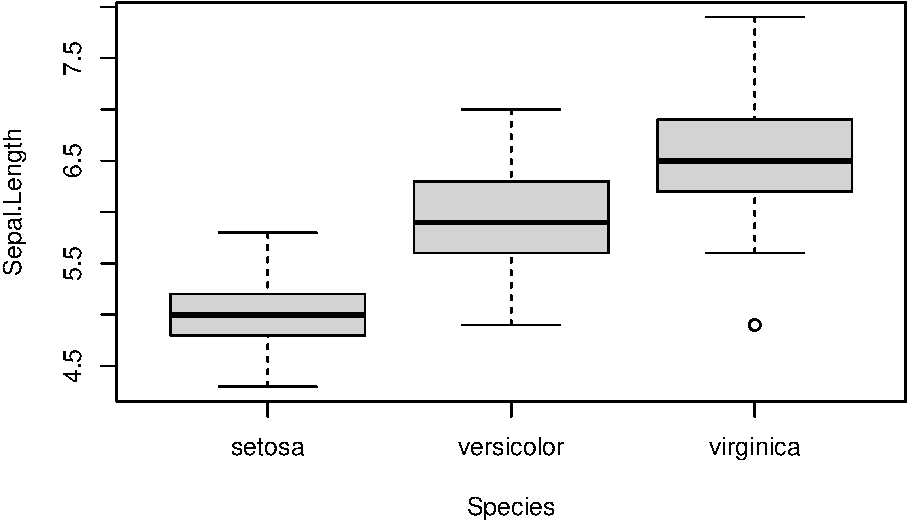
\includegraphics[keepaspectratio,alt={Sepal lengths for various species of iris.}]{figure/iris.plot-1.pdf}}
\caption{Sepal lengths for various species of iris.\label{fig:iris}}
\end{figure}

See figure~\ref{fig:iris}. (I am unsure why this is ``Fig. 1'' in the
caption\ldots is it a knitr/rmarkdown/pandoc thing, or a IEEEtran
thing?)

In practice, you will probably want to write your figure code in raw
\LaTeX~for greater control. In the setup chunk of this Rmd is a function
\texttt{latex.figure} which is an example of outputting raw \LaTeX~for a
figure. Tweak as you wish. (Surely there's a library like
\texttt{xtable} for this?)

\begin{Shaded}
\begin{Highlighting}[]
\FunctionTok{latex.figure}\NormalTok{(}
  \StringTok{\textquotesingle{}figure/iris.plot{-}1.pdf\textquotesingle{}}\NormalTok{,}
  \AttributeTok{caption=}\StringTok{\textquotesingle{}Another plot of sepal lengths}
\StringTok{           for the various species of iris.\textquotesingle{}}\NormalTok{,}
  \AttributeTok{label=}\StringTok{\textquotesingle{}fig:iris2\textquotesingle{}}\NormalTok{)}
\end{Highlighting}
\end{Shaded}

\begin{figure}[!t]%
\centering%
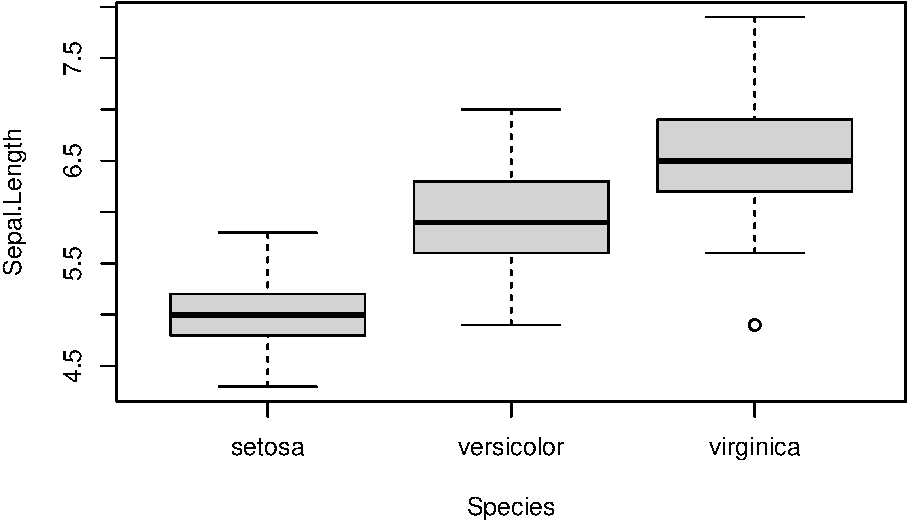
\includegraphics[width=\columnwidth]{figure/iris.plot-1.pdf}%
\caption{Another plot of sepal lengths
           for the various species of iris.}%
\label{fig:iris2}%
\end{figure}

The \texttt{latex.figure} also has basic support for subfloats: just
provide multiple paths. If there are as many captions as figures, one is
used for each. If there is one more than the number of figures, the
first is used as the ``master'' caption and the rest as subfigure
captions. If there is only one caption, it's used for the figure and no
subcaptions are added. See figure~\ref{fig:polynomials} for the result.

\begin{Shaded}
\begin{Highlighting}[]
\CommentTok{\# generate and save some pictures}
\NormalTok{n }\OtherTok{=} \DecValTok{1}\SpecialCharTok{:}\DecValTok{5}
\NormalTok{figs }\OtherTok{=} \FunctionTok{sprintf}\NormalTok{(}\StringTok{\textquotesingle{}figure/x\%i.png\textquotesingle{}}\NormalTok{, n)}
\ControlFlowTok{for}\NormalTok{ (nn }\ControlFlowTok{in}\NormalTok{ n) \{}
  \FunctionTok{png}\NormalTok{(}\AttributeTok{filename=}\NormalTok{figs[nn], }\AttributeTok{width=}\DecValTok{480}\NormalTok{, }\AttributeTok{height=}\DecValTok{300}\NormalTok{)}
  \FunctionTok{plot}\NormalTok{(}\DecValTok{1}\SpecialCharTok{:}\DecValTok{10}\NormalTok{, (}\DecValTok{1}\SpecialCharTok{:}\DecValTok{10}\NormalTok{)}\SpecialCharTok{\^{}}\NormalTok{nn)}
  \FunctionTok{dev.off}\NormalTok{()}
\NormalTok{\}}

\CommentTok{\# show as floating figure with 3 subfig}
\FunctionTok{latex.figure}\NormalTok{(}
\NormalTok{  figs,}
  \AttributeTok{caption=}\FunctionTok{c}\NormalTok{(}\StringTok{"Polynomials"}\NormalTok{,}
            \FunctionTok{sprintf}\NormalTok{(}\StringTok{"$x\^{}\%i$"}\NormalTok{, n)),}
  \AttributeTok{label=}\StringTok{\textquotesingle{}fig:polynomials\textquotesingle{}}\NormalTok{,}
  \AttributeTok{linebreaks.after=}\DecValTok{3}\NormalTok{,}
  \AttributeTok{width=}\StringTok{\textquotesingle{}.6}\SpecialCharTok{\textbackslash{}\textbackslash{}}\StringTok{columnwidth\textquotesingle{}}\NormalTok{,}
  \AttributeTok{floating=}\NormalTok{T)}
\end{Highlighting}
\end{Shaded}

\begin{figure*}[!t]%
\centering%
\subfloat[$x^1$]{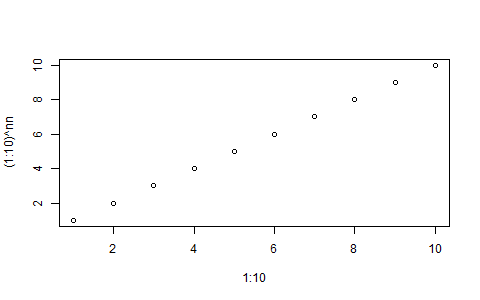
\includegraphics[width=.6\columnwidth]{figure/x1.png}}%
\subfloat[$x^2$]{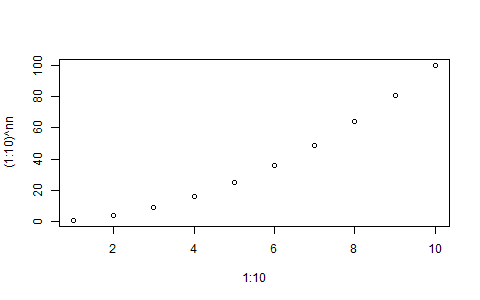
\includegraphics[width=.6\columnwidth]{figure/x2.png}}%
\subfloat[$x^3$]{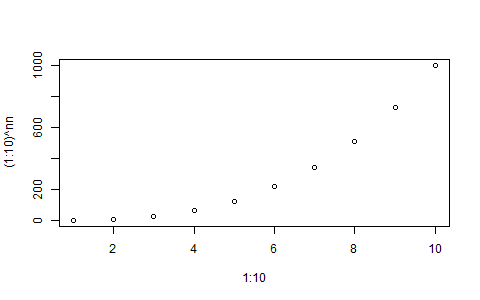
\includegraphics[width=.6\columnwidth]{figure/x3.png}}\\%
\subfloat[$x^4$]{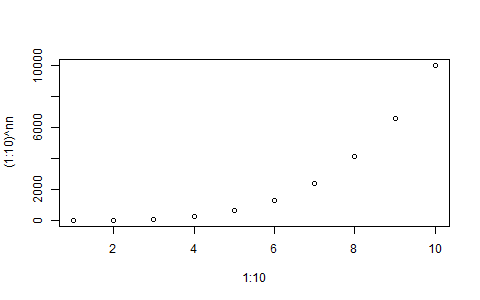
\includegraphics[width=.6\columnwidth]{figure/x4.png}}%
\subfloat[$x^5$]{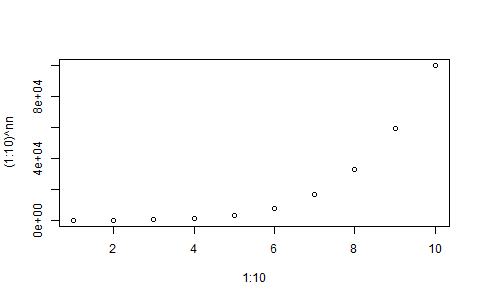
\includegraphics[width=.6\columnwidth]{figure/x5.png}}%
\caption{Polynomials}%
\label{fig:polynomials}%
\end{figure*}

Note that often IEEE papers with subfigures do not employ subfigure
captions, but instead will reference/describe all of them (a), (b),
etc., within the main caption.

Note that the IEEE typically puts floats only at the top, even when this
results in a large percentage of a column being occupied by floats.

\subsection{Tables}\label{sec:tables}

You should not use the pandoc syntax, because it uses the
\texttt{longtable} package (this is hard-coded in) and
\texttt{longtable} doesn't play well with two column input. Use
something like Hmisc or xtable to give \LaTeX~output and provide extra
control (e.g. table~\ref{tbl:iris.xtable}).

\begin{Shaded}
\begin{Highlighting}[]
\FunctionTok{print}\NormalTok{(}\FunctionTok{xtable}\NormalTok{(}
\NormalTok{  iris[}\FunctionTok{sample}\NormalTok{(}\FunctionTok{nrow}\NormalTok{(iris), }\DecValTok{6}\NormalTok{), ],}
  \AttributeTok{caption=}\StringTok{\textquotesingle{}Example of the iris dataset\textquotesingle{}}\NormalTok{,}
  \AttributeTok{label=}\StringTok{\textquotesingle{}tbl:iris.xtable\textquotesingle{}}\NormalTok{,}
  \AttributeTok{align=}\FunctionTok{c}\NormalTok{(}\FunctionTok{rep}\NormalTok{(}\StringTok{\textquotesingle{}r\textquotesingle{}}\NormalTok{, }\DecValTok{5}\NormalTok{), }\StringTok{\textquotesingle{}l\textquotesingle{}}\NormalTok{)))}
\end{Highlighting}
\end{Shaded}

\begin{table}[!t]
\centering
\caption{Example of the iris dataset} 
\label{tbl:iris.xtable}
\begin{tabular}{rrrrl}
  \hline
Sepal.Length & Sepal.Width & Petal.Length & Petal.Width & Species \\ 
  \hline
6.70 & 3.10 & 4.70 & 1.50 & versicolor \\ 
  5.40 & 3.00 & 4.50 & 1.50 & versicolor \\ 
  5.20 & 3.40 & 1.40 & 0.20 & setosa \\ 
  6.40 & 3.20 & 5.30 & 2.30 & virginica \\ 
  5.20 & 4.10 & 1.50 & 0.10 & setosa \\ 
  5.20 & 2.70 & 3.90 & 1.40 & versicolor \\ 
   \hline
\end{tabular}
\end{table}

You may wish the table to span multiple columns. Use \texttt{table*}
instead of \texttt{table} (table~\ref{tbl:xtable.floating}). Note that
the \texttt{floating.environment} is an argument to
\texttt{print.xtable}, not to \texttt{xtable}.

\begin{Shaded}
\begin{Highlighting}[]
\FunctionTok{print}\NormalTok{(}\FunctionTok{xtable}\NormalTok{(}
    \FunctionTok{head}\NormalTok{(mtcars),}
    \AttributeTok{caption=}\StringTok{\textquotesingle{}Example of the motor trend}
\StringTok{             car road tests dataset\textquotesingle{}}\NormalTok{,}
    \AttributeTok{label=}\StringTok{\textquotesingle{}tbl:xtable.floating\textquotesingle{}}\NormalTok{),}
  \AttributeTok{floating.environment=}\StringTok{\textquotesingle{}table*\textquotesingle{}}\NormalTok{)}
\end{Highlighting}
\end{Shaded}

\begin{table*}[!t]
\centering
\caption{Example of the motor trend
             car road tests dataset} 
\label{tbl:xtable.floating}
\begin{tabular}{rrrrrrrrrrr}
  \hline
mpg & cyl & disp & hp & drat & wt & qsec & vs & am & gear & carb \\ 
  \hline
21.00 & 6.00 & 160.00 & 110.00 & 3.90 & 2.62 & 16.46 & 0.00 & 1.00 & 4.00 & 4.00 \\ 
  21.00 & 6.00 & 160.00 & 110.00 & 3.90 & 2.88 & 17.02 & 0.00 & 1.00 & 4.00 & 4.00 \\ 
  22.80 & 4.00 & 108.00 & 93.00 & 3.85 & 2.32 & 18.61 & 1.00 & 1.00 & 4.00 & 1.00 \\ 
  21.40 & 6.00 & 258.00 & 110.00 & 3.08 & 3.21 & 19.44 & 1.00 & 0.00 & 3.00 & 1.00 \\ 
  18.70 & 8.00 & 360.00 & 175.00 & 3.15 & 3.44 & 17.02 & 0.00 & 0.00 & 3.00 & 2.00 \\ 
  18.10 & 6.00 & 225.00 & 105.00 & 2.76 & 3.46 & 20.22 & 1.00 & 0.00 & 3.00 & 1.00 \\ 
   \hline
\end{tabular}
\end{table*}

Note that, for IEEE style tables, given that table captions serve much
like titles, captions are usually capitalized except for words such as
a, an, and, as, at, but, by, for, in, nor, of, on, or, the, to and up,
which are usually not capitalized unless they are the first or last word
of the caption. Table text will default to
\texttt{\textbackslash{}footnotesize} as the IEEE normally uses this
smaller font for tables.

Note that the IEEE typically puts floats only at the top, even when this
results in a large percentage of a column being occupied by floats.

\subsection{Citing}\label{sec:citing}

Examples of citing one author \citep{Besag1974} and two authors
\citep{Besag1974, Besag1986}.

\subsection{Equations}\label{sec:equations}

Are as you would hope. You can use pandoc-crossref syntax to do labels.
i.e.

\begin{verbatim}
$$
e = m c^2
$$ {#eq:einstein}
\end{verbatim}

yields

\begin{equation}\protect\phantomsection\label{eq:einstein}{
e = m c^2.
}\end{equation}

One can use \texttt{@eq:einstein} to refer to the equation, e.g.
~\ref{eq:einstein}. The only caveat is that the equation needs to be in
its own paragraph if you wish to number it, meaning that in the
resultant tex and pdf, the equation is on its own line. (If you don't
wish to number the equation, it doesn't have to be on its own paragraph
and will render in the paragraph as you would expect).

I haven't found a good fix for this yet. It is a requirement of
\texttt{pandoc-crossref}. You have to go to the TeX and remove these
extra blank lines (where appropriate) before compiling. I add a comment
\texttt{\%\ FIXME\ ALIGNMENT} to these equations to make them easier to
find.

\section{Conclusion}\label{sec:conclusion}

Hopefully you have been given a brief tour of the capabilities of this
setup and will now go forth and author IEEEtran-style papers using
RMarkdown with (relative) ease.

\section*{Acknowledgement}\label{sec:acknowledgement}
\addcontentsline{toc}{section}{Acknowledgement}

This template would not be possible without
\href{https://www.ctan.org/tex-archive/macros/latex/contrib/IEEEtran/?lang=en}{Michael
Shell's IEEEtran files} \href{http://pandoc.org/}{pandoc},
\href{https://github.com/lierdakil/pandoc-crossref}{pandoc-crossref},
\href{http://yihui.name/knitr/}{knitr},
\href{http://rmarkdown.rstudio.com/}{rmarkdown}, and heavy googling
within \href{http://stackoverflow.com/}{StackOverflow}. And props to
\href{https://www.rstudio.com/}{Rstudio} too. It's not required for
this, but it certainly makes the whole process much easier. And anyone
else I forgot.

\bibliography{IEEEabrv,./library}

\end{document}
